\documentclass[tikz,border=60]{standalone}
\usepackage{tikz}
\usetikzlibrary{calc,shapes.callouts,shapes.arrows}

\definecolor{cadmiumgreen}{rgb}{0.0, 0.42, 0.24}
\definecolor{cobalt}{rgb}{0.0, 0.28, 0.67}
\definecolor{crimsonglory}{rgb}{0.75, 0.0, 0.2}
\definecolor{bleudefrance}{rgb}{0.19, 0.55, 0.91}
\definecolor{applegreen}{rgb}{0.1, 0.6, 0.0}
\definecolor{cadmiumred}{rgb}{0.89, 0.0, 0.13}
\definecolor{tangerine}{rgb}{0.95, 0.52, 0.0}
\definecolor{tangerine}{rgb}{0.95, 0.52, 0.0}
\definecolor{portlandorange}{rgb}{1.0, 0.35, 0.21}
\newcommand{\pointthis}[2]{
        \tikz[remember picture,baseline]{\node[anchor=base,inner sep=0,outer sep=0]%
        (#1);\node[overlay,rectangle callout,%
        callout relative pointer={(0.2cm,0.7cm)},fill=green!50] at ($(#1.north)+(-.5cm,-1.4cm)$) {#2};}%
        }%

\begin{document}
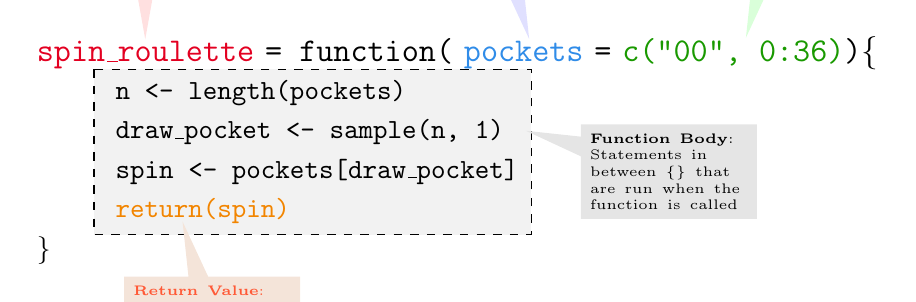
\begin{tikzpicture}
	
	\tikzstyle{process1} = [rectangle, minimum width=3cm, minimum height=1cm, text centered, draw=black, fill=red!10]
	\tikzstyle{process2} = [rectangle, minimum width=3cm, minimum height=1cm, text centered, draw=black, fill=blue!10]
	\tikzstyle{decision} = [diamond, minimum width=3cm, minimum height=1cm, text centered, draw=black, fill=black!10]
	\tikzstyle{arrow} = [thick,->,>=stealth]

\draw[dashed, fill = black!5] (0.85,-1.2) -- (0.85,-3.3) -- (6.4,-3.3) -- (6.4,-1.2) -- cycle;
	\node[anchor = west] at (0,-1) {\large{\color{cadmiumred}\texttt{spin\_roulette}} \texttt{= function(}
	{\color{bleudefrance}\texttt{pockets}} \texttt{=} {\color{applegreen}\texttt{c("00", 0:36)}}\texttt{)\{ }};
	
	\node[anchor = west] at (1,-1.5) {\texttt{n <- length(pockets)}};
	\node[anchor = west] at (1,-2) {\texttt{draw\_pocket <- sample(n, 1)}};
	\node[anchor = west] at (1,-2.5) {\texttt{spin <- pockets[draw\_pocket]}};
	\node[anchor = west] at (1,-3) {{\color{tangerine}\texttt{return(spin)}}};
	\node[anchor = west] at (0,-3.5) {\texttt{\}}};

	\node[overlay,rectangle callout,callout relative pointer={(-0.2cm,-0.7cm)},fill=green!15, text width=2cm] at (9.5,0.5) {\tiny{\color{cadmiumgreen}\textbf{Default Values:}\\ Values used if nothing is provided when the function is called}\\};
	
	\node[overlay,rectangle callout,callout relative pointer={(0.2cm,-0.7cm)},fill=blue!12, text width=2cm] at (6,0.5) {\tiny{\color{cobalt}\textbf{Parameters}:\\ Variables (inputs) that can be used in the function's body}\\};
	
	\node[overlay,rectangle callout,callout relative pointer={(0cm,-0.7cm)},fill=red!12, text width=2cm] at (1.5,0.5) {\tiny{\color{crimsonglory}\textbf{Function Name}:\\ Name of the function that can be called using \texttt{spin\_roulette()}}\\};
	
	\node[overlay,rectangle callout,callout relative pointer={(-0.2cm,0.7cm)},fill=red!70!green!15, text width=2cm] at (2.35,-4.45) {\tiny{\color{portlandorange}\textbf{Return Value}:\\ Output of your function computed within function body}\\};
	
	\node[overlay,rectangle callout,callout relative pointer={(-0.7cm,0.2cm)},fill=black!10, text width=2cm] at (8.15,-2.5) {\tiny{\color{black}\textbf{Function Body}:\\ Statements in between \{\} that are run when the function is called}\\};
	
\end{tikzpicture}
\end{document} 